\documentclass{article}
\usepackage[utf8]{inputenc}
\usepackage[margin=0.75in]{geometry}
\usepackage[colorlinks,linkcolor=blue]{hyperref}
\usepackage{cite}
\usepackage{listings}
\usepackage{float}
\usepackage{graphicx}
\usepackage[justification=centering]{caption}
\usepackage{subfigure} 
\usepackage{xcolor}
\lstset{language=python, %用于设置语言为bash
	keywordstyle=\color{blue!70}\bfseries, %设置关键词为蓝色,需要引xcolor宏包
	basicstyle=\small,
	commentstyle=\ttfamily, %基本和注释的字体都使用默认的等宽,而非texlive调用的中文字体
	showstringspaces=false, %不显示中间的空格
	frame=shadowbox,  %边框
}

\begin{document}
	\begin{center}
    
    	% MAKE SURE YOU TAKE OUT THE SQUARE BRACKETS
    
		\LARGE{\textbf{Robotics 2020: Project Report}} \\
		(intermediate and final)\\
        \vspace{1em}
        \Large{Project name: Efficient Point-Cloud Semantic Segmentation} \\
        \small{"A project of the 2020 Robotics Course of the School of Information Science and Technology (SIST) of ShanghaiTech University \\ 
        \url{https://robotics.shanghaitech.edu.cn/teaching/robotics2020}”}\\
        \vspace{1em}
        \normalsize\textbf{Delin Feng, Longtian Qiu, Qianjing Shi} \\
        \normalsize{fengdelin@cau.edu.cn, qiult@shanghaitech.edu.cn, shiqj@shanghaitech.edu.cn} \\
        \vspace{1em}
        \normalsize{Advisor: Sören Schwertfeger, Yijun Yuan} \\
        \vspace{1em}
     
	\end{center}
    \begin{normalsize}
    
    	\section{Abstract:}
        LiDAR point-cloud segmentation is an important problem for many applications. For large-scale point cloud segmentation, there are four paradigms for semantic segmentation: projection-based, discretization(voxel) based, point-based, and hybrid methods. Voxel-based representation is regular and has good memory locality. However, it requires very high resolution in order not to lose information. Point-based 3D modeling methods are memory efficient. but it lacks the local context modeling capability. Projection-based methods discover that the feature distribution of LiDAR images changes drastically at different image locations. This project will propose an algorithm merging the advantages of different methods to solve the problem of missing detailed structure and pose after projection or down-sampling to improve the efficiency and accuracy of the algorithm. Inspired by the voxel structure of Cylinder3D, multilayer processing of the original point cloud data is carried out on the basis of project-based method, so that it has the advantages similar to voxel. We will conduct experiments on some open source data sets such as SemanticKITTI and compare results with state of the art methods to evaluate the performance of the algorithm. We will also create our own(ShanghaiTech campus) data set for experiments to verify the efficiency and accuracy of the algorithm.    \\
      
		\section{Introduction:}
        
        Efficient semantic segmentation of 3D point clouds is a fundamental and essential capability for real-time intelligent systems, such as autonomous driving and augmented reality, also it can provide more semantic information. Recently, deep learning has been shown to be very effective for point cloud perception tasks. Conventionally, researchers rasterize the point cloud into voxel grids and process them using 3D volumetric convolutions. With low resolutions, there will be information loss during voxelization: multiple points will be merged together if they lie in the same grid. Therefore, a high-resolution representation is needed to preserve the fine details in the input data. However, the computational cost and memory requirement both increase cubically with voxel resolution. Another stream of models attempt to directly process the input point clouds. These point-based models require much lower GPU memory than voxel-based models thanks to the sparse representation. However, they neglect the fact that the random memory access is also very inefficient. Projection-based methods can perform semantic segmentation more quickly, but are limited by the fuzzification of CNN output and discretization errors. In order to achieve semantic segmentation of point clouds on autonomous mobile robots, we will process point clouds based on SqueezeNet to obtain 2d images, and implement further feature fusion based on the point-voxel framework to improve the current lack of detailed structure and some of the reprojection problem. Since there is less open source data for point cloud semantic segmentation, we plan to collect data from the ShanghaiTech campus for experiments, but because the point cloud ground truth calibration is very troublesome, this is a difficult challenge for us.\\
        Our key challenges are: 1)How to improve efficiency of projection-based method, it will not worse then current method. 2)Voxel method has more requirements on memory, so it’s important to improve details under the guarantee of current quality.
        
	   	\section{State of the Art:}
        
      Find literature and open-source-ROS packages relevant to your project. Per team member:
       
\begin{itemize}
   
\item Fengdelin's proposal:
\\
"Deep Learning for 3D Point Clouds: A Survey"\cite{9127813} is a survey of existing methods of 3D point cloud semantic segmentation, "PointSeg: Real-Time Semantic Segmentation Based on 3D LiDAR Point Cloud" uses end-to-end point-based method to improve the segmentation performance.\cite{2018PointSeg}
\\
The pvcnn paper\cite{pvcnn} first talked about the disadvantages of voxel-based and point-based methods. Voxel-based representation is regular and has good memory locality. However, it requires very high resolution in order not to lose information. Point-based 3D modeling methods are memory efficient. it lacks the local context modeling capability, this will lead to the irregular memory access pattern and introduce the dynamic kernel computation overhead, which becomes the efficiency bottlenecks.\\
PV-Conv contains two branches, one is point-based and the other is Voxel-based.
The first steps of voxel-based branch operations are similar to most voxel-based methods, including normalizing coordinates, voxelization, apply a stack of 3D volumetric convolutions to aggregate the features. If Only here, there will still be problems of resolution and loss of detial information, so the article uses point-based branch to introduce geometric detail information very cleverly to supplement the deficiencies of voxel-based;
One of the highlights of this article is deoxelization. Its function is to convert the features of a voxel into the features of each point in the voxel. The article considers that the feature of each voxel corresponds to the center of each voxel, and uses the trilinear interpolation method to ensure that the features of each point are different. It seems a bit Like deconvolution in 2d deep learning.\\
The point-based method no longer uses the points of the neighborhood, but uses MLP to directly calculate the feature of each point.\\
With both individual point features and aggregated neighborhood information, it can efficiently fuse two branches with an addition as they are providing complementary information.\\
\\
We maybe will use ROS Velodyne\_pointcloud package to collect our own 3D point cloud dataset.\\
This package provides point cloud conversions for Velodyne 3D LIDARs and provides 4 ROS nodes and nodelets: CloudNodelet, CloudNodelet, cloud\_node, transform\_node. \\
Theses nodes reads raw data from the velodyne\_packets ROS topic, converts to sensor\_msgs/PointCloud2 format, and republishes to velodyne\_points ROS topic in the original frame of reference (typically /velodyne). In addition to the XYZ points, this cloud includes fields for "intensity" and "ring".
You can transform raw Velodyne packets into sensor\_msgs/PointCloud2 messages into the /odom frame.\\
We plan to use velodyne to obtain the school’s 3d point cloud data and perform experimental processing. With this ros package, you can view lidar data pointcloud2 on rviz for visualization and quantitative analysis of experimental effects.\\
\item Qiulongtian's proposal:\\
In paper \emph{SqueezeSegV2}\cite{wu2019squeezesegv2}, they introduce a new model SqueezeSegV2 that is more robust to dropout noise in LiDAR point clouds. In paper \emph{Rangenet++}\cite{milioto2019rangenet++}, they focus  more on LiDAR-only semantic segmentation forward in order to provide another independent source of semantic information to the vehicle. 
\\\\
To be more specific, in paper \emph{SqueezeSeg}\cite{wu2018squeezeseg}, they address semantic segmentation of road-objects from 3D LiDAR point clouds, particularly for cars and pedestrians. Focusing on road-object segmentation so we use (Velodyne style) 3D LiDAR point clouds. Given point cloud output from a LiDAR scanner, the task aims to isolate objects of interest and predict their categories. To feed 3D point clouds to a 2D CNN, it adopt a spherical projection to 
transform sparse, irregularly distributed 3D point clouds to dense, 2D grid representations. The proposed CNN model draws inspiration from SqueezeNet  and is carefully designed to reduce parameter size and computational complexity, with an aimto reduce memory requirements and achieve real-time inference speed for our target embedded applications, which is very similar to our aims. In 3D projection to asphere, we shouldn’t ignore something important, which they also mention but they hadn’t tackled with.
\\
For package, I recommend ROS velodyne\_laserscan package, which is design to extract a single ring of a Velodyne PointCloud2 and publish it as a LaserScan message. In our project, we may need to process a small part of the point cloud so this package may be helpful in our development.

\item Shiqianjing's proposal:\\
In paper \emph{PointNet++(Deep Hierarchical)}\cite{qi2017pointnet++}, they introduced a hierarchical neural network that applies PointNet recursively on a nested partitioning of the input point set,called PointNet ++, which is able to learn deep point set features efficiently and robustly. Here\cite{qi2017pointnet},they provide analysis towards understanding of what the network has learned and why the network is robust with respect to input perturbation and corruption.\\

However, I want to introduce this paper in detail, \emph{Fully-convolutional point networks for large-scale point clouds}\cite{rethage2018fully}. Because it focus on efficiently processing large-scale 3D data. And in our project, we do need to collect data of 3D and is in large-scale.In contrast to conventional approaches that maintain either unorganized or  organized representations, from input to output, its approach has the advantage of operating on memory efficient input data representations while at the same time exploiting the natural structure of convolutional operations to avoid the redundant computing and storing of spatial information in the network. Besides, it can produce either an ordered output or map predictions directly onto the input cloud, thus making it suitable as a general-purpose point cloud descriptor applicable to many 3D tasks. In our project, when we transfer a 3D-sphere into its projection, we will meet many problems in projection of how to tackle with the fact that small objects will be projected so small and computer is hard to recognize them so that they may be ignored. However, sometimes they are really important object-s such as pedestrians. As we all know, in autonomous driving, how to keep cars away them is a big question to keep pedestrians safe. So if we ignore data of pedestrians, it will cause big problem.
\\\\
For package, I prefer velodyne\_driver in my paper. This is a ROS 2 driver for Velo-dyne devices. It currently supports the 64E(S2, S2.1, S3), the 32E, the 32C, and the VLP-16. This driver is responsible for taking the data from the Velodyne and  combining it into one message per revolution. If we want to turn that raw data into a pointcloud or laserscan, we can see the velodyne\_pointcloud and velodyne\_laserscan packages.This package provides basic device handling for Velodyne 3D LIDARs. For a list of all supported models refer to the Supported Devices section. The driver publishes device-dependent velodyne\_msgs/VelodyneScan data. This driver supports all current Velodyne HDL-64E, HDL-32E, VLP-32C, and VLP-16 models. There is little difference in the way it handles those devices. For our project, we will use some data collecting from campus using 32-beam Lidar, which scans the whole campus. So I think this package is very important to our project.\\
      ~\\

\end{itemize}
      \emph{Add}: For intermediate, we add one more paper which is very relevant to our problem as we also use some code in it to test our own model, which is SqueezeSegV3\cite{xu2020squeezesegv3}. LiDAR point-cloud segmentation is an important problem for many applications. For large-scale point cloud segmentation, the defacto method is to project a 3D point cloud to get a 2D LiDAR image and use convolutions to process it. Despite the similarity between regular RGB and LiDAR images, the feature distribution of LiDAR images changes drastically at different image locations. Using standard convolutions to process such LiDAR images is problematic, as convolution filters pick up local features that are only active in specific regions in the image. As a result, the capacity of the network is under-utilized and the segmentation performance decreases. To fix this, authors in the paper proposed Spatially-Adaptive Convolution (SAC) to adopt different filters for different locations according to the input image. SAC can be computed efficiently since it can be implemented as a series of element-wise multiplications, im2col, and standard convolution. It is a general framework such that several previous methods can be seen as 
      special cases of SAC. Recent work on point-cloud segmentation is mainly divided into two categories, focusing on small-scale or large-scale point-clouds. For small-scale problems, ranging from object parsing to indoor scene understanding, most of the recent methods are based on PointNet. Although PointNet-based methods have achieved competitive performance in many 3D tasks, they have limited processing speed, especially for large-scale point clouds. For outdoor scenes and applications such as autonomous driving, typical LiDAR sensors, such as Velodyne HDL-64E LiDAR, can scan about 64 × 3000 = 192, 000 points for each frame, covering an area of 160×160×20 meters. Processing point clouds at such scale efficiently or even in real time is far beyond the capability of PointNetbased methods. Hence, much of the recent work follows the method based on spherical projection. Instead of processing 3D points directly, these methods first transform a 3D LiDAR point cloud into a 2D LiDAR image and use 2D ConvNets to segment the point cloud. As shown In this paper, we follow this method based on spherical projection. 
      By reference to SAC, it provides us a fresh view of convolution of pointclouds. We can learn from it can improve our model.
 


    	\section{System Description:}
        
         For large-scale point cloud segmentation, there are four paradigms for semantic segmentation: projection-based, discretization(voxel)based, point-based, and hybrid methods. Among them, the projection-based method is often more suitable for automatic driving and autonomous mobile robots. In our project, we plan to project a 3d point cloud in spherical coordinates based on the SqueezeSeg framework to obtain a 2d image. Semantic segmentation of the image is carried out through the deep neural network, and then the image is remapped to 3d to obtain the 3d point cloud after semantic segmentation. However,projection, this intermediate representation inevitably brings several problems such as discretization errors and occlusions.Because the 3d point cloud is projected to 2d, it will produce some details information loss. And after predicting the label for each pixel, once the labels are projected into the original point clouds, two or more points stored in the same range of image pixels will obtain the same semantic label. \\
         The existing solutions to the problem of the lack of down-sampling detail information include Rangenet++ using range information to reconstruct to three dimensions, and using effective point labels KNN search. SqueezeSeg combines the CNN image prediction results and the original point cloud data into CRF to refine the label map. PointSeg uses dilated convolutional layers to obtain multi-scale features and broaden the receptive field. RandLA-Net expands the receptive field by dilated residual block.\\
         Our current rough idea is to combine the depth map to supplement the detailed information on the basis of the projection-based method, and consider the point-voxel (PVCNN) architecture to extract features more effectively. \\
         First, we combined the SqueezeSegV3 projection-based method and RandLA's\cite{Hu2019RandLA} point-based method, and added the feature map of SqueezeSeg to RandLa. This direct feature fusion also needs to consider the size of the feature and this method is not an end-to-end solution. In the following code, $priors$ is a feature generated by SqueezesegV3 and is fused in RandLA. After experimental verification, the effect of this method is better than SqueezeSegV3 and RandLA to a certain extent, especially on people, bicycles, motorcycles and other small objects.\\
         \begin{lstlisting}
         cloud_ind = int(np.argmin(self.min_possibility))
         pick_idx = np.argmin(self.possibility[cloud_ind])
         pc_path = path_list[cloud_ind]
         pc, tree, labels, priors = self.get_data(pc_path)
         selected_pc, selected_labels, selected_idx = self.crop_pc(pc, labels, tree, pick_idx)
         selected_priors = priors[selected_idx]
         
         # update the possibility of the selected pc
         dists = np.sum(np.square((selected_pc -pc[pick_idx]).astype(np.float32)), axis=1)
         delta = np.square(1 - dists / np.max(dists))
         self.possibility[cloud_ind][selected_idx] += delta
         self.min_possibility[cloud_ind] = np.min(self.possibility[cloud_ind])
         
         if True:
         yield (selected_pc.astype(np.float32),
         selected_labels.astype(np.int32),
         selected_priors.astype(np.int32),
         selected_idx.astype(np.int32),
         np.array([cloud_ind], dtype=np.int32))
         \end{lstlisting}
         
         Second, we consider a method that combines the projected image and the original point for feature fusion, and regards the projected image as a layer of voxels, which contains the original point cloud projected to the same area, and combines the work of PVCNN to fuse the features. Currently, inspired by the voxel structure of Cylinder3D, multilayer processing of the original point cloud data is carried out on the basis of project-based method, so that it has the advantages similar to voxel. Multi-layered improvements can supplement missing information at different distances. The following code implements the hierarchical operation based on distance and supplements the detailed structure at different locations.
         \begin{lstlisting}
         if i==0:
         d_s=0
         else:
         d_s=depth_max/(self.layer_num+1-i)
         
         d=depth[depth>=d_s]
         #print(proj_x.shape)
         proj_x = proj_x[depth>=d_s]
         # round and clamp for use as index
         proj_x = np.floor(proj_x)
         proj_x = np.minimum(self.proj_W - 1, proj_x)
         proj_x = np.maximum(0, proj_x).astype(np.int32)   # in [0,W-1]
         if i==0:
         self.proj_x =np.copy(proj_x)  # store a copy in orig order
         
         proj_y = proj_y[depth>=d_s]
         proj_y = np.floor(proj_y)
         proj_y = np.minimum(self.proj_H - 1, proj_y)
         proj_y = np.maximum(0, proj_y).astype(np.int32)   # in [0,H-1]
         if i==0:
         self.proj_y = np.copy(proj_y)  # stope a copy in original order
         
         # order in decreasing depth
         indices = np.arange(d.shape[0])
         order = np.argsort(d)[::-1]
         depth = d[order]
         indices = indices[order]
         points = self.points[order]
         remission = self.remissions[order]
         proj_y = proj_y[order]
         proj_x = proj_x[order]
         # assing to images
         self.proj_range[i,proj_y, proj_x] = depth
         self.proj_xyz[i,proj_y, proj_x] = points
         self.proj_remission[i,proj_y, proj_x] = remission
         self.proj_idx[i,proj_y, proj_x] = indices
         self.proj_mask = (self.proj_idx> 0).astype(np.int32)
         \end{lstlisting}
         \begin{lstlisting}
         proj = torch.cat([proj_range.unsqueeze(0).clone(),#proj_range.unsqueeze(0).clone(),
         proj_xyz.clone().permute(3,0,1,2),#proj_xyz.clone().permute(2,0,1),
         proj_remission.unsqueeze(0).clone()])
         #proj_remission.unsqueeze(0).clone()])
         proj=proj.reshape(proj.shape[0]*proj.shape[1],proj.shape[2],proj.shape[3])
         sensor_img_means=[]
         sensor_img_stds=[]
         
         sensor_img_means=self.sensor_img_means.repeat(scan.layer_num)
         sensor_img_stds=self.sensor_img_stds.repeat(scan.layer_num)
         #sensor_img_stds=self.sensor_img_stds.repeat(scan.layer_num)
         proj = (proj - sensor_img_means[:,None,None]) / sensor_img_stds[:,None,None]
         proj = proj * proj_mask.float()
         \end{lstlisting}
         
         ~\\
         ~\\
         \\
         Since we will scan data in campus, let’s first introduce our equipment first.\\
         Jackal is a robot car which carries Velodyne’s VLP-16 sensors. Jackal is a rugged, lightweight, fast, and easy-to-use unmanned ground vehicle for ROS Indigo, presented by Clearpath Robotics, including a standard internal PC, as well as basic IMU and GPS. Standard perception modules are available, including URDF and simulator integration, and demonstration applications. \\
         The Core packages are: jackal\_control ,jackal\_description, jackal\_msgs, jackal\_navigation.\\
         Others are jackal\_desktop: jackal\_viz, jackal\_robot: jackal\_base-jackal\_bringup, jackal\_simulator: jackal\_gazebo.\\
         ~\\
         If we want to scan data outside, we want to make the robot move first. To visualize it, we connect it to a screen, mouse and a keyboard so that we can see the desktop of Jackal. We went to the Robotics Lab many times because there were many problems and each time we went to the lab we could finally overcame it. First, we did spend several weeks as the robot car has some strange problems as it can’t move. After taking a good battery from other place to our Jackal, the indicator light is on. To control Jackal with PS3 handshake, we need Bluetooth module and Jackal’s Ubuntu System doesn’t have so we search some code and install it by ourselves. “\emph{\$ sudo make install INTERFACE=usb}”, after that, input “\emph{\$ hciconfig}” to confine whether out PS3 handle is recognized by Ubuntu. Then input “\emph{\$ hciconfig hci0 up}”, “\emph{\$ bluetoothctl}” so we can connect with the handle. However, we found that there sill remained some strange problems that although we type the right code, Jackal kept still. But what we have found strangely is that as long as there are some problems we can’t overcome with many tries, next time we can fix it with the same solution automatically with high probability. To start Jackal, we use code “\emph{\$ roslaunch jackal\_base  base.launch}”, and start control module by “\emph{\$rosrun teleop\_twist\_keyboard teleop\_twist\_keyboard.py}”. Right now, Jackal can move and so we focused on the Velodyne-16. Since the former one on it is a more expensive on, so we replace it with a 16-beam-detector as professor required. \\
         ~\\
         Velodyne’s VLP-16 sensor is the smallest, newest and most advanced production Velodyne’s 3D LiDAR product range. Vastly more cost-effective than similarly priced sensors and developed with mass production in mind, it retains the key features of Velodyne’s breakthroughs in LiDAR: Real-time, 360°, 3D distance and calibrated reflectivity measurements. The VLP-16 has a range of 100m, and the sensor’s low power consumption (\~{}8W), lightweight (500-gram or 830-gram options available), compact footprint (\~{}Ø103mm x 72mm), and dual return capability make it ideal for UAVs and other mobile applications.Velodyne’s LiDAR VLP-16 supports 16 channels, \~{}300,000 points/sec, a 360° horizontal field of view and a 30° vertical field of view, with \~{}15° up and down. The Velodyne VLP-16 does not have visible rotating parts, making it highly resilient in challenging environments (Rated IP67). \\
         ~\\
         Next part is scanning data and visualization, which can show the point clouds scanned by Velodyne in Rviz by running code “\emph{\$ rosrun rviz rviz -f velodyne}; \emph{\$ roslaunch velodyne\_pointcloud VLP16\_points.launch rosbag record velodyne\_points}”. To experiment our code late, we record it and save it so we can use SqueezeSeg V3’s code to test our model.\\
         To this point, we were finally well-prepared to scan data. But as we don’t have a screen so we install Sunlogin remote control on both Jackal and laptop so that we can supervise what is scanning when Jackal was moving, and record at anytime we wanted.\\
         Finally we succeeded and scanned some point clouds data underground of SIST building, with pedestrians, roads, cars and some motorbikes.\\
         ~\\
         Right now we have the original file that is \emph{.bag} file. However the code of SqueezeSegV3 requires \emph{.bin} file. So in terminal we first transform it into \emph{.pcd} file.
         \begin{lstlisting}
         # terminal1
         roscore

         # terminal2
         mkdir pcd
         cd pcd
         rosrun pcl_ros pointcloud_to_pcd input:=/velodyne_points

         # terminal 3
         rosbag play input_file.bag
         \end{lstlisting}
         Then change it to \emph{.bin} file through the python code as follow.
         \begin{lstlisting}
         import numpy as np
         import os

         def read_pcd(pcd_path):
            lines = []
            num_points = None

            with open(pcd_path, 'r') as f:
                for line in f:
                    lines.append(line.strip())
                    if line.startswith('POINTS'):
                        num_points = int(line.split()[-1])
            assert num_points is not None

            points = []
            for line in lines[-num_points:]:
                x, y, z, i, r = list(map(float, line.split()))
                points += [x, y, z, i]

            return points


         if __name__ == '__main__':
            files = None

            for root, dirs_name, files_name in os.walk("./pcd"):
                files = files_name

            for f_name in files:
                pcd_points = read_pcd("./pcd/" + f_name)

                total = np.array(pcd_points, dtype=np.float32)
                total.tofile('./result/{}.bin'.format(f_name[:-4]))
         \end{lstlisting}
         Finally we get \emph{.bin} file and we put it in the model trained by authors of SqueezeSegV3 to test and predict. Since the pre-trained model provided by the author of Sv3, it’s trained based on KITTI dataset, which is collected by HDL-64 and ours is Velodyne-16. So we have to shrink the projection-image from 64*2048 to 16*1024 to make sure that the graph is continuous.As a result, the graph is blur and loses details. So the prediction from the CNN works poorly and we can only see part of the motorcycle is labeled. Prediction graphs are shown below.
         \begin{figure}[htbp]
            \centering
            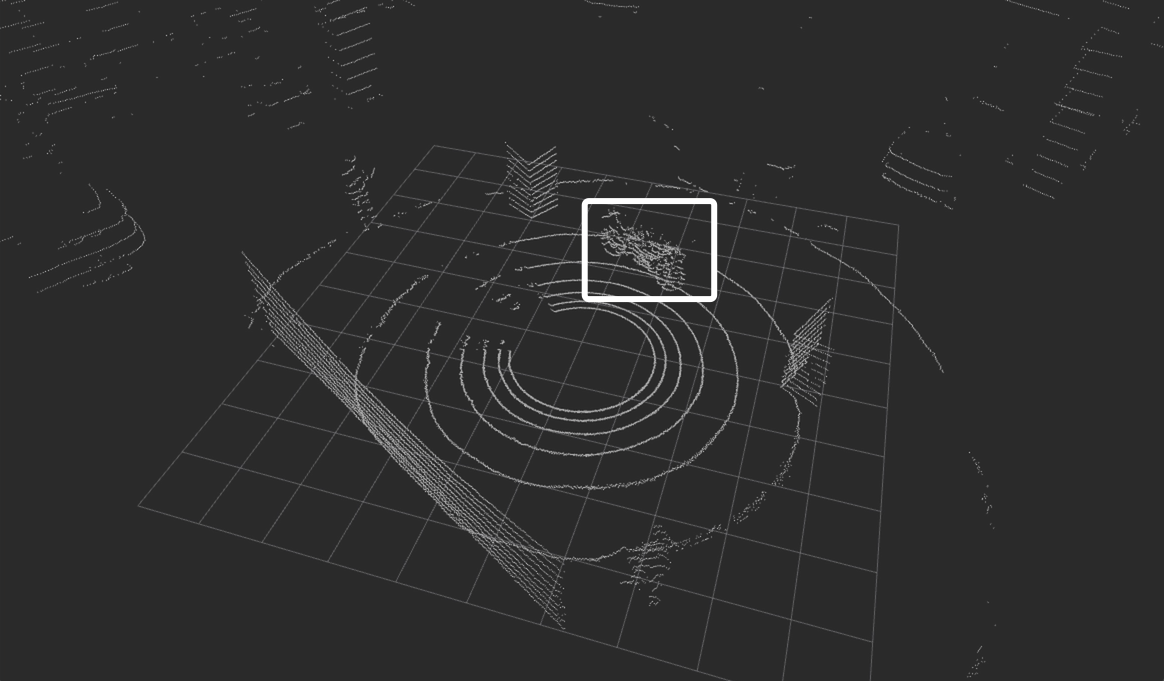
\includegraphics[width=9cm]{pointc1.png}
            \quad
            
\includegraphics[width=9cm ,height = 2cm]{pointc2.png}
            \quad
            \caption{Pointcloud and SqueezeSeg Result}
        \end{figure}

          \begin{figure}[htbp]
          \centering
          \subfigure[Ours\_mul]{
            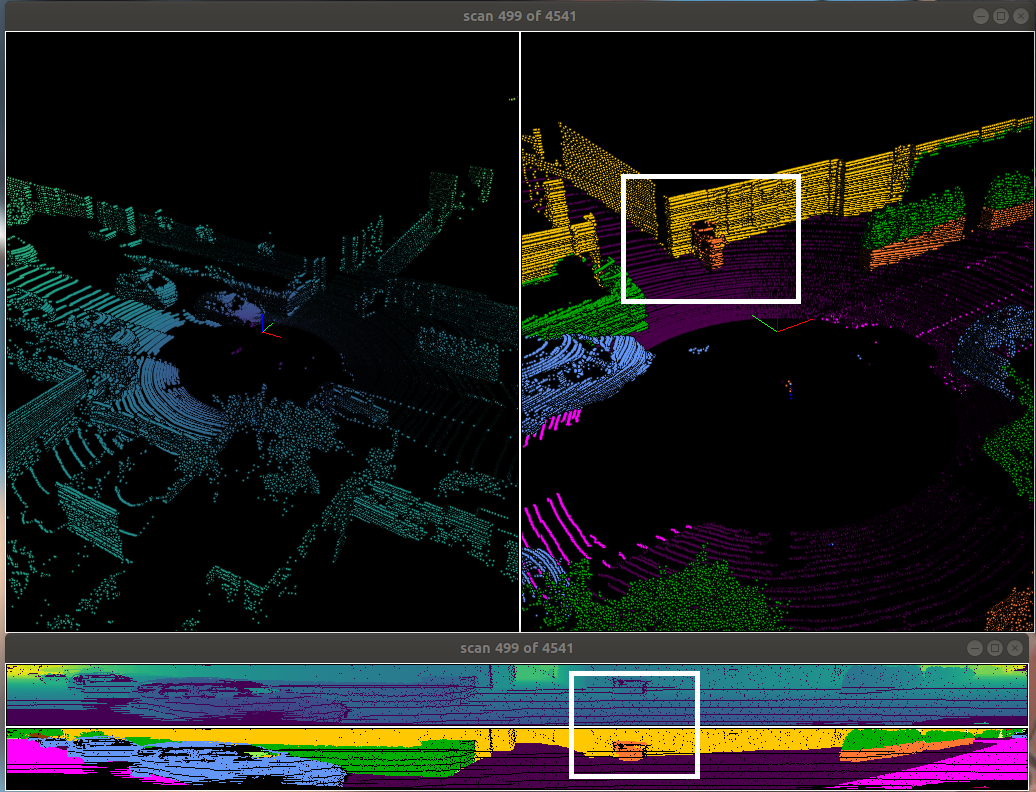
\includegraphics[width=9cm]{m1.png}
            %\caption{fig1}
          }
          \quad
          \subfigure[SqueezeSeg.]{
            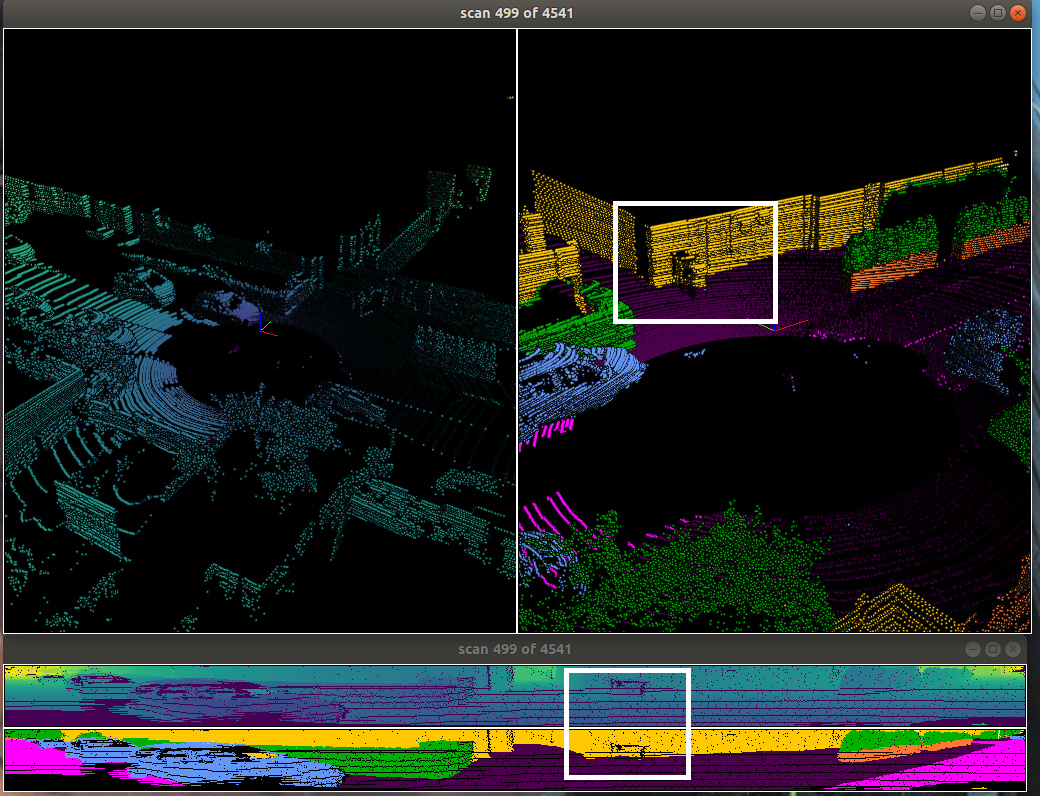
\includegraphics[width=9cm]{m2.png}
          }
          \quad
          \subfigure[GroundTruth.]{
            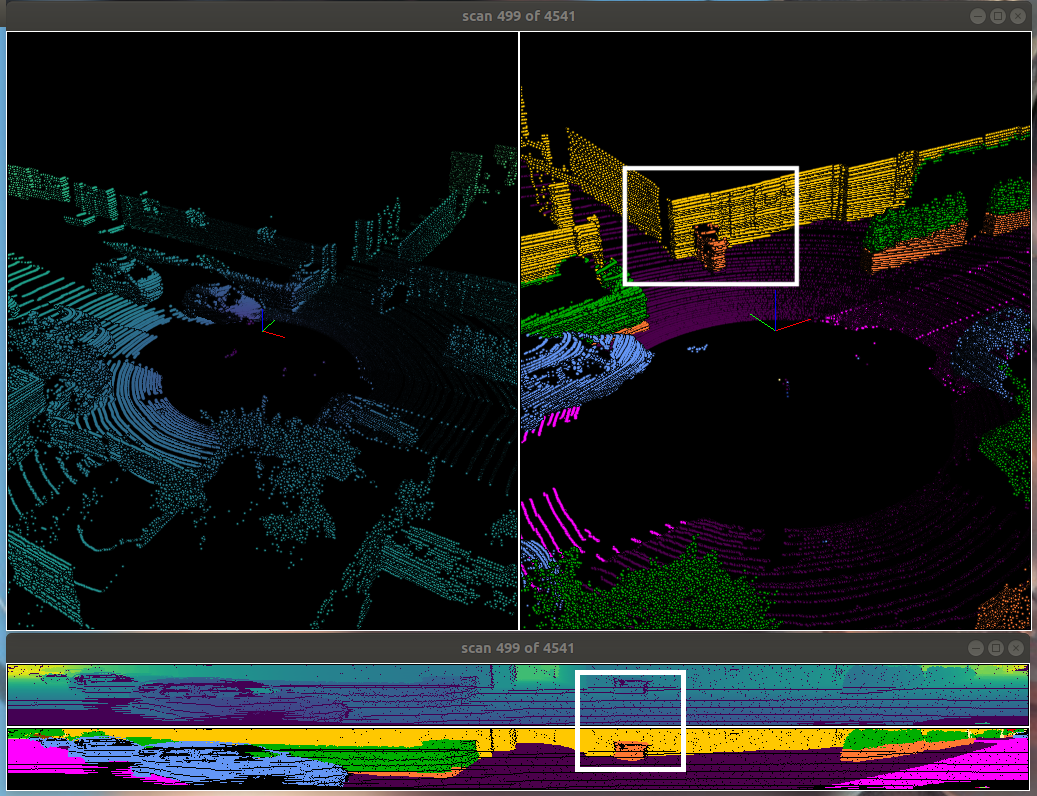
\includegraphics[width=9cm]{m3.png}
          }
          \quad
          \caption{Effect comparison\\The upper left corner of the image is the original point cloud, the upper right corner is the output semantic point cloud, and the lower part is the projected image and semantic segmentation image of the point cloud}
        \end{figure}
        
                 

    	\section{ System Evaluation: }
        The evaluation of the system is divided into two parts: qualitative and quantitative evaluation. The qualitative evaluation will use our scanned 3D point cloud of the ShanghaiTech University campus to visualize the effect. Quantitative evaluation will be performed on the SemanticKITTI dataset. After using our algorithm to predict the validation set, we will submit our results to SemanticKITTI’s semantic segmentation competition to obtain mean Jaccard or so-called intersection-over-union (mIoU)) over all classes, accuracy. We will compare with some of the current advanced algorithms, mainly with projection-based methods to compare the recognition accuracy of different categories, overall accuracy, running time, memory consumption, etc.\\
        Currently our algorithm has achieved initial progress, point and projection model accuracy and benefiting all above SqueezeSegV3 and RandLA, small objects in people, bicycles, motorcycles, such as easy on the types of error identification recognition effect also has the improvement (and because of the work force is limited, at present we have trained for only 3 epoch, and the maximum number of epoch RandLA default is 100, we believe that to continue training performance will be better. See Table 1.\\
        \begin{table}[h] %h表示三线表在当前位置插入
        	%\setlength{\abovecaptionskip}{0.05cm} %设置三线表标题与第一条线间距
        	\centering
        	\caption{\textbf{The results comparison}} 
        	%表头文本加黑,但不加黑Table 1.字样,引入包即可:\usepackage[labelfont=bf]{caption}
        	\begin{tabular*}{\hsize}{@{\extracolsep{\fill}}c c cccccccc} %{\hsize}使三线表自适应宽度,c表示文本居中
        		\hline
        		methods & accurancy & mIoU&car&bicycle&motorcycle&truck&other-vehicle&person&bicyclist\\
        		\hline 
        		SqueezeSeg53 &0.891&0.527&0.861&0.309&0.478&\textbf{0.507}&\textbf{0.424}&0.522&0.524\\
        		RandLA &0.899 &0.539& \textbf{0.942}&0.260&0.258&0.401&0.389&0.492&0.482\\
        		Ours1& \textbf{0.903}&\textbf{0.543}&0.9277&\textbf{0.3627}& \textbf{0.5108}&0.3181&0.3649&\textbf{0.5532}&\textbf{0.6267} \\
        		Ours\_mul &0.885&0.504&0.862&0.220&0.469&0.377&0.388&0.383&0.474\\
        		\hline
        	\end{tabular*}
        \begin{tabular*}{\hsize}{@{\extracolsep{\fill}}c c ccccccc} %{\hsize}使三线表自适应宽度,c表示文本居中
        	\hline
        	methods &motorcyclist&road&parking&sidewalk&other-ground&building&fence\\
        	\hline 
        	SqueezeSeg53 &0.000&0.945&0.473&\textbf{0.816}&0.003&0.802&0.472 \\
        	RandLA &0.00&0.907&\textbf{0.603}&0.737&0.204&\textbf{0.869}&\textbf{0.563}\\
        	Ours1 &0.00&0.9341&0.3903&0.7997&\textbf{0.366}&0.8575&0.4211  \\
        	Ours\_mul &0.000&\textbf{0.9445}&0.479&0.808&0.006&0.807&0.523 \\
        	\hline
        \end{tabular*}
    \begin{tabular*}{\hsize}{@{\extracolsep{\fill}}c c ccccccc} %{\hsize}使三线表自适应宽度,c表示文本居中
    	\hline
    	&vegetation&trunk&terrain&pole&traffic-sign\\
    	\hline 
    	SqueezeSeg53 &0.825&0.525&0.720&0.424&0.382 \\
    	RandLA &0.814&\textbf{0.613}&0.668&0.492&0.477\\
    	Ours1 &\textbf{0.8667}&0.5881&\textbf{0.7442}& 0.5839&0.4224   \\
    	Ours\_mul &0.809&0.504&0.692&0.419&0.313 \\
    	\hline
    \end{tabular*}
        \end{table}
        
        At present, the multi-layer projection model can supplement the details of remote objects. Since the current multi-layer model has not been refined, post-processed and optimized, some losses of other parts will be caused. We're going to improve on that. Meanwhile, due to limited computing power, the default batch size of SqueezeSeg was 8, while our algorithm used 4, which also affected the segmentation effect.\\
        From Figure 2, we can see that the multi-layer model supplements the details of the long distance according to the distance. The distance of the lidar point cloud is usually some larger objects, such as buildings, fences, and roads. Therefore, in the results of Table 1, the partitioning effect of buildings, fences, and roads is better, which is improved on the basis of SqueezeSeg.\\

        SqueezeSeg and Ours\_mul in Table 1 are based on the projection method, the other two are the results of post-processing, except for the results of RandLA which are based on the test set, the other three are based on the results of the validation set. Therefore, the result of Ours1 may be relatively high.
        

       \section{Conclusions:}
        In this paper, we will propose SqueezeSeg as our projection-based method without bad segmentation performance than the original SqueezeSeg. We believe it can be used as a general-purpose feature descriptor by evaluating it on challenging benchmarks at different scales, namely semantic scene and part-based object segmentation. Overall, we hope our approach will be able to outperforms the state of the art both in accuracy and run time. Maybe our research can be a new way to optimize semantic segmentation for autonomous vehicles and robots. 
        
    

\end{normalsize}
 \bibliographystyle{plain}
 \bibliography{ref}
\end{document}
